\documentclass{beamer}
\usetheme{Warsaw}
\usecolortheme{seahorse}
\usepackage{amsmath}
\usepackage{amsfonts}
\usepackage{amssymb}
%\usepackage{CJKutf8}
\title{Introduction to Fourier Transform and Signal Analysis}
\author{\texorpdfstring{Zong-han, Xie\newline\url{icbm0926@gmail.com}}{Zong-han, Xie}}
\begin{document}
%\begin{CJK}{UTF8}{cwmc}
\begin{frame}
\titlepage
\end{frame}
\begin{frame}[label=licensepage]
\frametitle{License of this document}
Introduction to Fourier Transform and Signal Analysis by Zong-han, Xie (\href{icbm0926@gmail.com}{icbm0926@gmail.com}) is licensed under a Creative Commons Attribution-NonCommercial 4.0 International License. \newline
\begin{center}
\includegraphics[scale=1]{by-nc-sa.eps}
\end{center}
\end{frame}
\AtBeginSection[]
{
  \begin{frame}
    \frametitle{Outline}
    \tableofcontents[currentsection]
  \end{frame}
}
\section{Continuous Fourier Transform}
\begin{frame}
\frametitle{Orthogonal Condition}
\begin{itemize}
\item Any two vectors $\mathbf{a}$, $\mathbf{b}$ satisfied the following condition are mutually orthogonal. \newline
\begin{eqnarray}
\mathbf{a}^* \cdot \mathbf{b} = 0
\label{eq:ortho_vec}
\end{eqnarray}
\item Any two functions $a(x)$, $b(x)$ satisfied the following condition are mutually orthogonal. \newline
\begin{eqnarray}
\int{a^*(x)} \cdot {b(x)} dx = 0
\label{eq:ortho_func}
\end{eqnarray}
\item * means complex conjugate. \newline
\end{itemize}
\end{frame}
\begin{frame}
\frametitle{Complete and Orthogonal Basis}
\begin{itemize}
\item $\cos nx $ and $\sin mx$ are mutually orthogonal in which n and m are integers.
\begin{eqnarray}
\int_{-\pi}^{\pi}{\cos nx} \cdot {\sin mx} dx = 0 \nonumber \\
\int_{-\pi}^{\pi}{\cos nx} \cdot {\cos mx} dx = \pi\delta_{nm} \nonumber \\
\int_{-\pi}^{\pi}{\sin nx} \cdot {\sin mx} dx = \pi\delta_{nm}
\end{eqnarray}
\item $\delta_{nm} $ is Dirac-delta symbol. It means $\delta_{nn} = 1$ and $\delta_{nm} = 0$ when $n \neq m$.
\end{itemize}
\end{frame}
\begin{frame}
\frametitle{Fourier Series}
Since $\cos nx $ and $\sin mx$ are mutually orthogonal, we can expand an arbitrary periodic function $f(x)$ by them. we shall have a series expansion of $f(x)$ which has $2\pi$ period.
\begin{eqnarray}
f(x)&=&a_0 + \sum_{k=1}^{\infty} \left(a_k\cos kx + b_k \sin kx\right) \nonumber \\
a_0&=&\frac{1}{2\pi}\int_{-\pi}^{\pi}f(x) dx \nonumber \\
a_k&=&\frac{1}{\pi}\int_{-\pi}^{\pi}f(x) \cos kx dx \nonumber \\
b_k&=&\frac{1}{\pi}\int_{-\pi}^{\pi}f(x) \sin kx dx
\label{eq:fseries}
\end{eqnarray}
\end{frame}
\begin{frame}
\frametitle{Fourier Series}
If $f(x)$ has $2L$ period instead of $2\pi$, $x$ is replaced with $\pi x /L$.
\begin{eqnarray}
f(x)&=&a_0 + \sum_{k=1}^{\infty} \left(a_k\cos kx + b_k \sin kx\right) \nonumber \\
a_0&=&\frac{1}{2L}\int_{-L}^{L}f(x) dx \nonumber \\
a_k&=&\frac{1}{L}\int_{-L}^{L}f(x) \cos kx dx \nonumber \\
b_k&=&\frac{1}{L}\int_{-L}^{L}f(x) \sin kx dx
\label{eq:fseries_pL}
\end{eqnarray}
\end{frame}
\begin{frame}
\frametitle{Complex Fourier Series}
Using Euler's formula, equation (\ref{eq:fseries}) becomes 
\begin{eqnarray}
f(x)=a_0 + \sum_{k=1}^{\infty} \left(\frac{a_k - ib_k}{2} e^{ikx} + \frac{a_k + ib_k}{2}e^{-ikx}\right) \nonumber
\end{eqnarray}
Let $c_0 \equiv a_0$, $c_k \equiv \frac{a_k - ib_k}{2}$ and $c_{-k} \equiv \frac{a_k + ib_k}{2}$, we have
\begin{eqnarray}
f(x)=\sum_{m=-\infty}^{\infty} c_m e^{imx}
\label{eq:cfseries}
\end{eqnarray}
$e^{imx}$ and $e^{inx}$ are also mutually orthogonal provided $n \neq m$ and it forms a complete set. Therfore, it can be used as orthogonal basis.
\end{frame}
\begin{frame}
\frametitle{Fourier Series of Step Function}
$f(x)$ is a periodic function with $2\pi$ period and it's defined as follows.
\begin{eqnarray}
f(x)&=& 0, -\pi < x < 0 \nonumber \\
f(x)&=& h, 0 < x < \pi
\label{eq:stepfunc}
\end{eqnarray}
Fourier series of $f(x)$ is
\begin{eqnarray}
f(x)= \frac{h}{2} + \frac{2h}{\pi} \left( \frac{\sin x}{1} + \frac{\sin 3x}{3} + \frac{\sin 5x}{5} + ...\right)
\label{eq:stepfunc_ft}
\end{eqnarray}
$f(x)$ is piecewise continuous within the periodic region. Fourier series of $f(x)$ converges at speed of $1/n$.
\end{frame}
\begin{frame}
\frametitle{Fourier Series of Step Function}
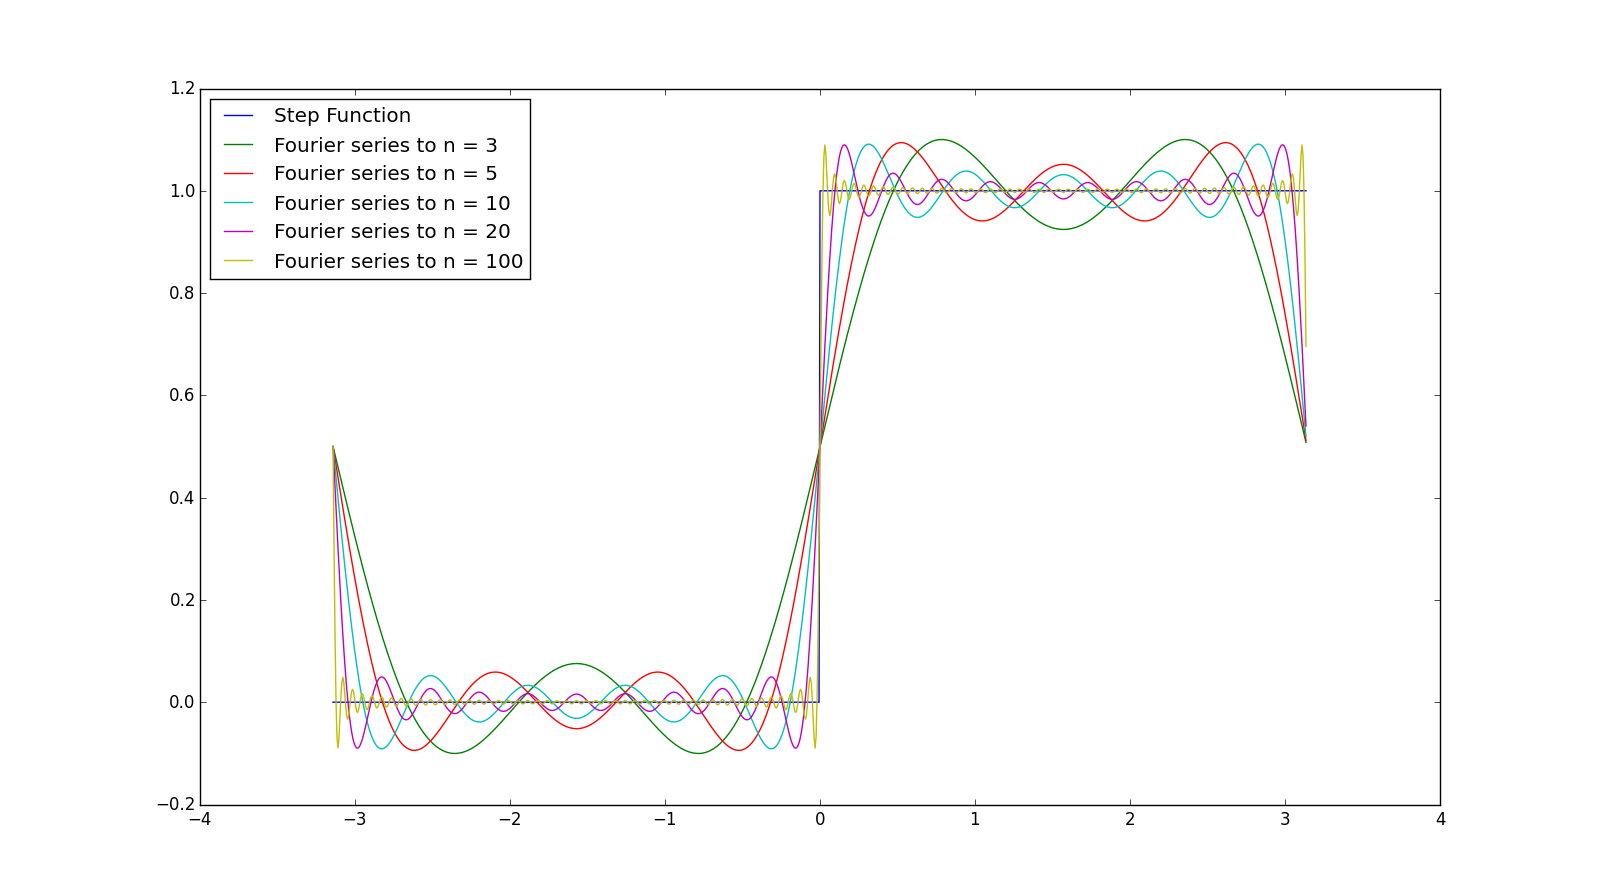
\includegraphics[scale=0.3]{step.png}
\end{frame}
\begin{frame}
\frametitle{Fourier Series of Saw Tooth Function}
$f(x)$ is a periodic function with $2\pi$ period and it's defined as follows.
\begin{eqnarray}
f(x)&=& -x, -\pi < x < 0 \nonumber \\
f(x)&=& x, 0 < x < \pi
\label{eq:sawfunc}
\end{eqnarray}
Fourier series of $f(x)$ is
\begin{eqnarray}
f(x)= \frac{\pi}{2} - \frac{4}{\pi} \sum_{n=1,3,5...} \left( \frac{\cos nx}{n^2} \right)
\label{eq:sawfunc_ft}
\end{eqnarray}
$f(x)$ is continuous and its derivative is piecewise continuous within the periodic region. Fourier series of $f(x)$ converges at speed of $1/n^2$.
\end{frame}
\begin{frame}
\frametitle{Fourier Series of Saw Tooth Function}
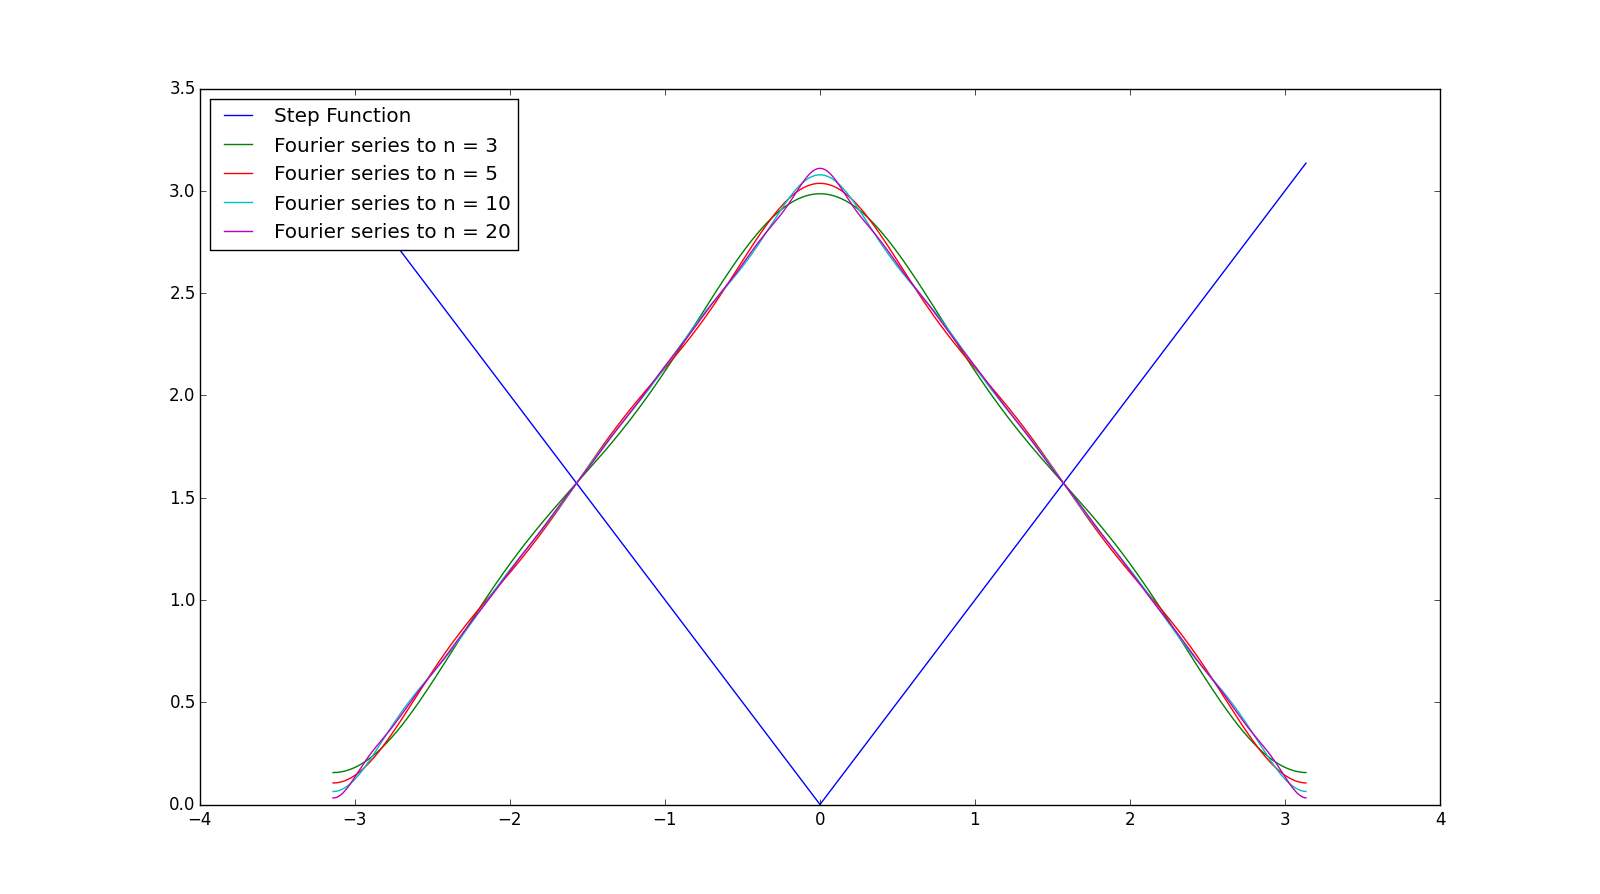
\includegraphics[scale=0.3]{sawtooth.png}
\end{frame}
\begin{frame}
\frametitle{Fourier Series of Full Wave Rectifier}
$f(t)$ is a periodic function with $2\pi$ period and it's defined as follows.
\begin{eqnarray}
f(t)&=& -\sin {\omega t}, -\pi < t < 0 \nonumber \\
f(t)&=& \sin {\omega t}, 0 < t < \pi
\label{eq:fullrectifier_func}
\end{eqnarray}
Fourier series of $f(x)$ is
\begin{eqnarray}
f(t)= \frac{2}{\pi} - \frac{4}{\pi} \sum_{n=2,4,6...} \left( \frac{\cos n\omega t}{n^2 - 1} \right)
\label{eq:fullrectifier_func_ft}
\end{eqnarray}
$f(x)$ is continuous and its derivative is piecewise continuous within the periodic region. Fourier series of $f(x)$ converges at speed of $1/n^2$.
\end{frame}
\begin{frame}
\frametitle{Fourier Series of Full Wave Rectifier}
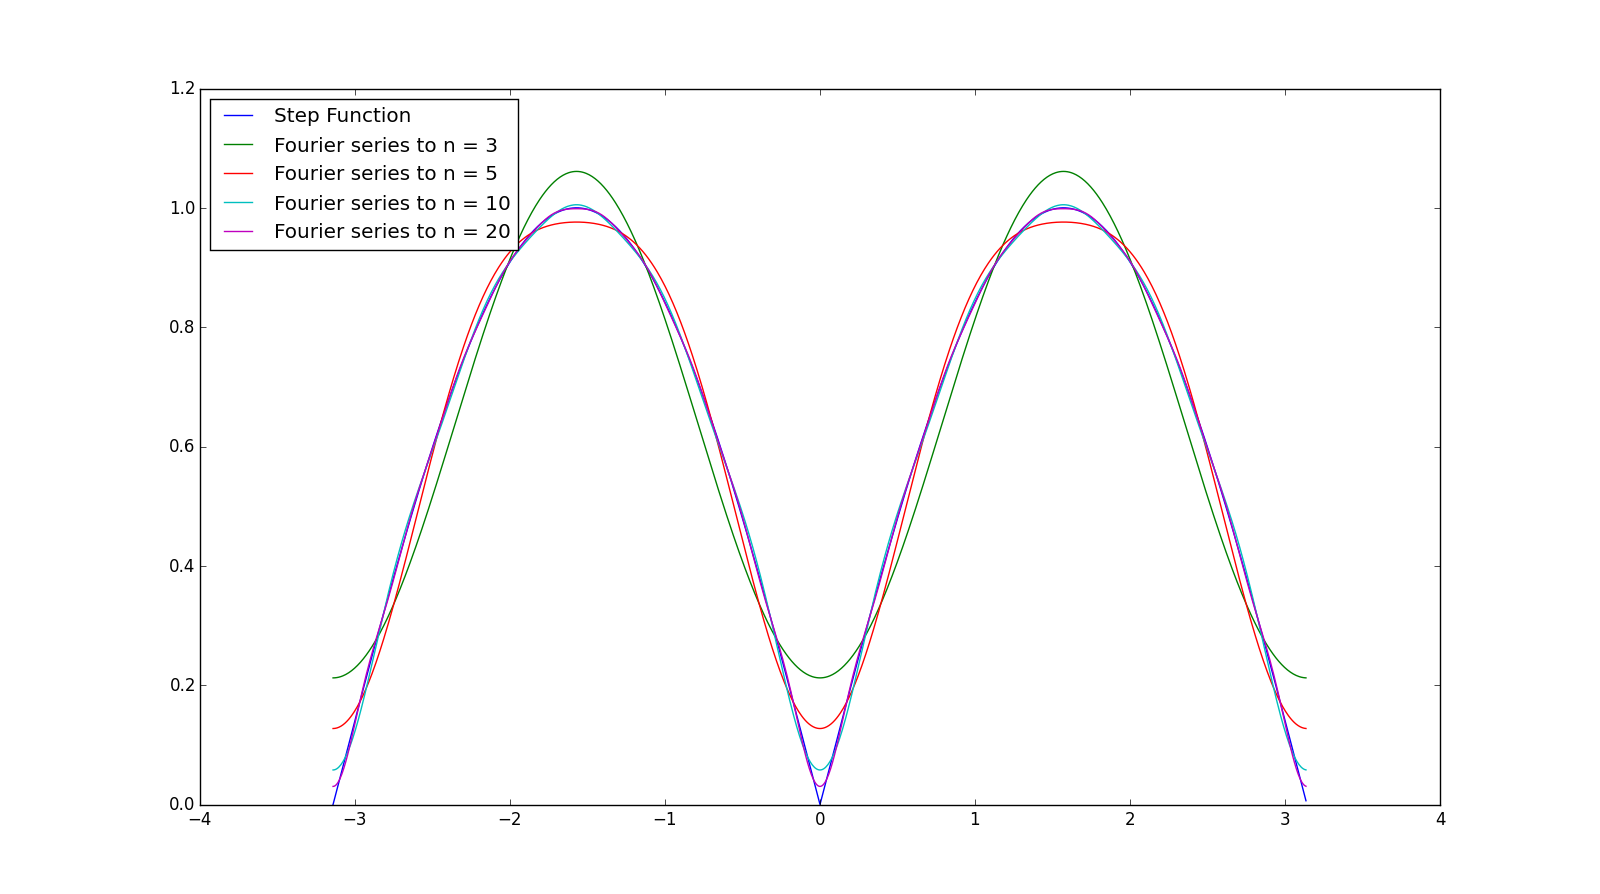
\includegraphics[scale=0.3]{fullrectifier.png}
\end{frame}
\begin{frame}
\frametitle{Fourier Transform}

\end{frame}
\begin{frame}
\frametitle{Convolution Theory and Parseval Relation}
\end{frame}
\begin{frame}
\frametitle{Fourier Transform of a Gaussian Function}
\end{frame}
\begin{frame}
\frametitle{Fourier Transform of a Gaussian Function with Carrier}
\end{frame}
\begin{frame}
\frametitle{Transfer Function}
\end{frame}
\section{Discrete Fourier Transform}
\begin{frame}
\frametitle{From Continuous to Discrete Fourier Transform}
\end{frame}
\begin{frame}
\frametitle{Frequency Bins and Nyquist Frequency}
\end{frame}
\begin{frame}
\frametitle{Concept of Nyquist-Shannon Frequency}
\end{frame}
\begin{frame}
\frametitle{Aliasing}
\end{frame}
\begin{frame}
\frametitle{Window Functions}
\end{frame}
\begin{frame}
\frametitle{Filter}
\end{frame}
\begin{frame}
\frametitle{Fast Fourier Transform}
\end{frame}
\section{Calculate DFT with Python Numpy Package}
\begin{frame}
\frametitle{Discrete Fourier Transform in Numpy or Scipy}
\end{frame}
\begin{frame}
\frametitle{Transform One Dimensional Data}
\end{frame}
\begin{frame}
\frametitle{Transform More than One Dimensional Data}
\end{frame}
\section{References}
\begin{frame}
\frametitle{References}
\begin{itemize}
\item \url{http://idv.sinica.edu.tw/jwang/SNGP/SNGP20090621.pdf}
\item MATHEMATICAL METHODS FOR PHYSICISTS by George B. Arfken and Hans J. Weber. ISBN-13: 978-0120598762
\item Numerical Recipes 3rd Edition: The Art of Scientific Computing by William H. Press  (Author), Saul A. Teukolsky. ISBN-13: 978-0521880688
\item Chapter 12 and 13 in \url{http://www.nrbook.com/a/bookcpdf.php}
\end{itemize}
\end{frame}
\section{}
%---------------Examples of Latex---------
\begin{frame}
\frametitle{2nd page}
\begin{block}{block}
\begin{eqnarray}
\frac{1}{2}
\end{eqnarray}
\end{block}
\begin{alertblock}{alertblock}
alertblock content
\end{alertblock}
\end{frame}
\begin{frame}
\frametitle{3rd page}
\begin{itemize}
\item<1-> 第一
\item<1-> 2nd
\item<2-> 3rd
\item<3-> etc.
\hyperlink{1stpage}{\beamerbutton{go fuck}}
\end{itemize}
\end{frame}
%\end{CJK}
\end{document}
